%!TEX root = main.tex
\begin{figure*}[ht!]
\centering
\vspace{-15pt}
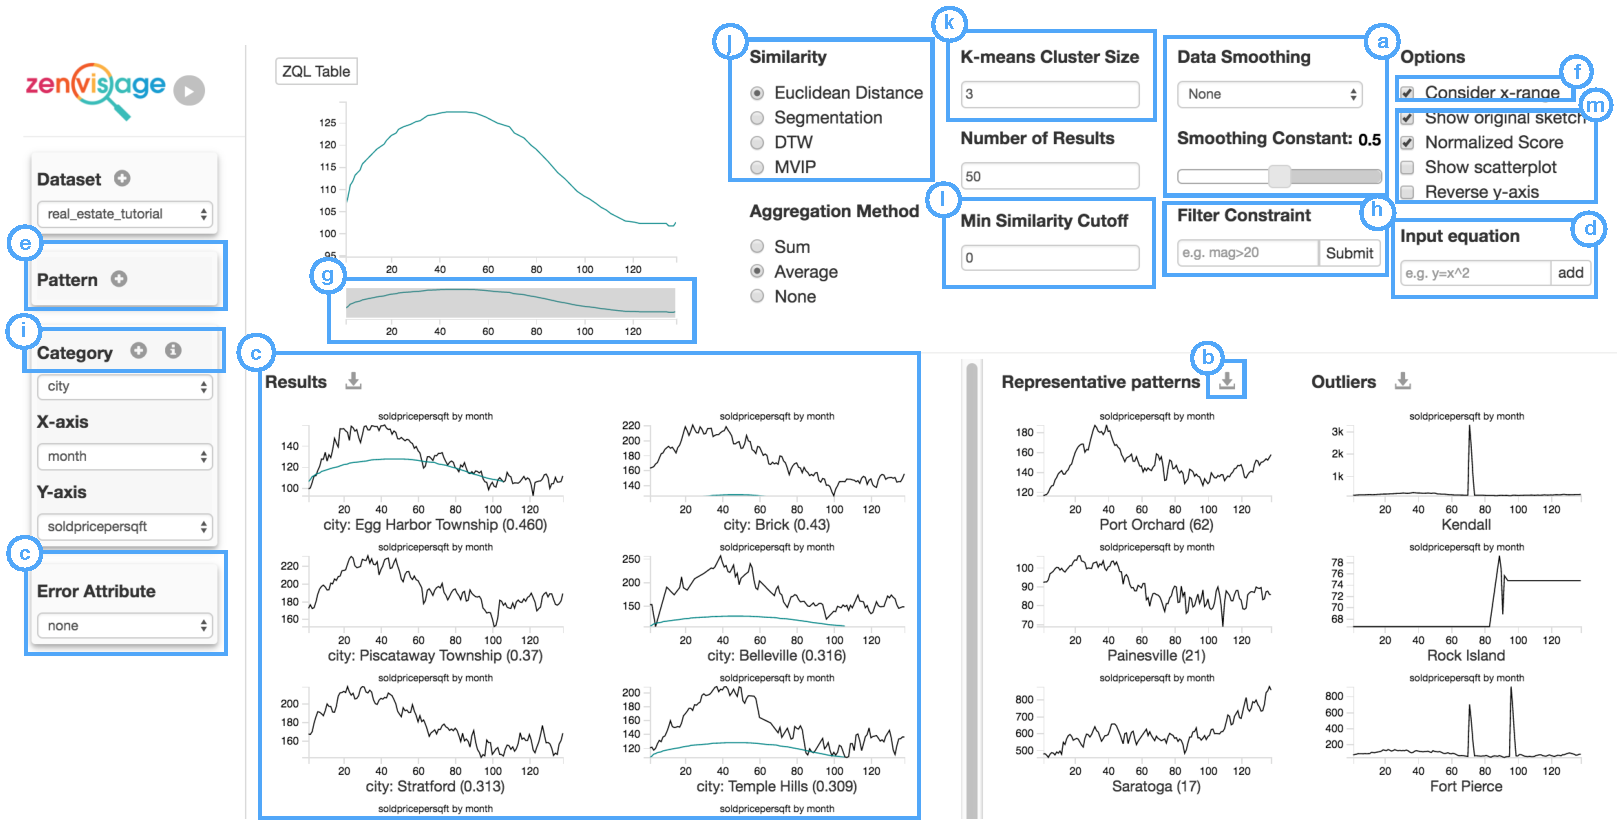
\includegraphics[width=\linewidth]{figures/newZV.pdf} %5.5
\vspace{-5pt}\caption{Our VQS after participatory design, which includes: the ability to preprocess via (a) interactive smoothing; (b, c) the ability to export data outputs ; querying functionalities via (d) equations and (e) patterns; query specification mechanisms including (f) x-range invariance, (g) x-range selection and filtering, (h) Filtering, and (i) Dynamic class creation; (j, k, l) system parameter options; (m) visualization display options. Prior to the participatory design, \zv only included a single sketch input with no additional options. \zv also displayed representative patterns and outlier patterns, as shown in Figure~\ref{oldZV}.}
\label{zvOverview}
\vspace{-14pt}
\end{figure*}
\section{Themes Emerging from Participatory Design (RQ2)}\label{findings}
\par In the previous section, we gained an understanding of the current analysis workflows employed in the three use cases. Next, to address RQ2, we employed participatory design with our scientists to incorporate key features  missing in our original VQS, and unaddressed in their
current workflows. We discovered three central themes encapsulating these features that are important to facilitate rapid hypothesis generation and insight discovery, but are missing in prior VQSs. While some of our findings echo prior work on system-level taxonomies of visualization tasks \cite{Amar2005,Heer2012}, we highlight how specific analytic tasks and interaction features could be used to enhance VQSs in particular. \techreport{In particular, we learned that \textit{participants wanted more control over the internals of the systems and an integrated workflow that helped streamline their analysis when using VQSs.}}
\subsection{Uninterrupted workflow}
\par Our cognitive walkthroughs revealed that in many participants' existing workflows, they switched between parameter specification, code execution, and visualization comparisons. The non-interactive nature of these segmented workflows has been shown to incur a large cognitive barrier during exploratory data analysis \cite{Kery2017}. In addition, since scientific research often takes place in a collaborative setting, this means that the data sense-making process could be delayed by weeks because the analysis-to-results phases needed to be rerun offline based on changes that were suggested during a meeting. Moreover, data-cleaning emerged as a common pain-point, echoing prior work~\cite{kandel2011wrangler,Kandel2012}.

%%%%%%%%%%%%%%%%%%%%%%%%%%%%%%%%%

\stitle{Integrative preprocessing through interactive smoothing:} While \zv does not attempt to solve all of the pre-processing issues that we faced during participatory design, we identified data smoothing as a common data cleaning procedure that could benefit from a tight integration between pre-processing and visual analysis. \tvcg{\npar Data smoothing is a denoising procedure that generates a smoothed pattern approximating key features of the visualized trend with less noise. Smoothing also raises an interesting trade-off between the smoothness of the curve and the quality of shape-matching for VQSs. If the visualization is over-smoothed, then shape matching would return results that only loosely resemble the query pattern. However, if no smoothing is applied, then the noise may dominate the overall trend, which could also lead to bad pattern matches. In addition, it is often hard to tell what the appropriate smoothing parameter should be applied simply by visualizing a small number of sampled visualization, as one would do in an offline analysis.}
%\kk{We don't need to define this -- a citation would suffice.} %\dor{I think this paragraph is important to keep to reflect why smoothing is not a one-shot operation and how it works with the querying functionalities of the system, perhaps need to shorten this.}}
\npar To address this issue, we developed an interface for users to interactively adjust the data smoothing algorithm and parameters on-the-fly to update the resulting visualizations accordingly (Figure \ref{zvOverview}a). This was applied to the \matsci and \astro use cases, as both had noisy and dense observational data. 

%%%%%%%%%%%%%%%%%%%%%%%%%%%%%%%%%
\stitle{Facilitating export for downstream analysis:} Since \tvcg{VQSs are designed to be exploratory tools that suggest potential directions for further analysis, rather than for performing one-shot operations, we asked participants how they envisioned themselves using VQSs in their workflow}. Both the \astro and \bio participants wanted to use VQSs as a way to identify interesting objects or characteristic patterns, which they will later feed into a more advanced downstream pipeline. 
\npar To smoothen the transition between the VQS and their downstream analysis, we implemented export functionalities for downloading the similarity, representative trend and outlier results as csv files (Figure \ref{zvOverview}b). Individual visualizations can also be downloaded by double-clicking individual figures (Figure \ref{zvOverview}c) to facilitate easier sharing of visualization results with collaborators. 
%%%%%%%%%%%%%%%%%%%%%%%%%%%%%%%%%%%%%%%%%%%%%%%%%%%%%%%%%%%%%%%%%%%%%%%%%%%%%%%%%%%%%%%%%%%%%%%%%%%% 
%\subsection{Sophisticated data operations in a VQS}
\tvcg{\subsection{Increasing expressiveness of querying capabilities}}
%%%%%%%%%%%%%%%%%%%%%%%%%%%%%%%%%
% The initial VQS did not satisfy the participants' needs for sophisticated data operations. They wanted more expressive ways to explore their data, either through additional querying methods, or the ability to query on a subset of data.
\par While the interactions in our original prototype enabled simple visual queries, many scientists were interested in extending their querying capabilities, either through different querying modalities or through more flexible query specification methods.  

\stitle{Input Equations:} Our \matsci participants expressed that some solvents can have analytical models that characterize the relationships between chemical properties. They wanted to find solvents that satisfied these relationships. We implemented a feature that plots a given function (e.g. $y=x^2$) on the canvas, which is then used as input for similarity search (Figure \ref{zvOverview}d).

\stitle{Upload Pattern as Query:} While the input equation is useful when simple analytical models exist, this may not be true for other domains. In these cases, users can upload a query pattern of a sequence of points (Figure \ref{zvOverview}e). This is useful for patterns generated from advanced computational models used for understanding scientific processes, usually as part of the downstream analysis of the exploratory workflow. %For example, the \bio team are trying to develop a time series prediction algorithm using machine learning based on some biological parameters \cite{Peng2016}. For the \astro team, it is also common to compare synthetic light curves generated from simulations against observations \cite{Nugent1997}.

\stitle{Consider/Ignore x-range:} We improved query specification by allowing users to change how the shape-matching criterion is applied. For finding supernovae, A1 primarily cared about the existence of a peak above a certain amplitude with an appropriate width of the curve, rather than the exact time that the event occurred, leading them to use the consider x-range feature. G1 also expressed that she does not really know what is the ``trigger point'' of when the expression level of a gene will rise and it would be interesting to find all ``rising'' profiles independent of the change-point.  We implemented an option to ignore the x-range in shape matching (Figure \ref{zvOverview}f) and a brushing mechanism that enables users to select the specific x-region they want to perform their shape matching on (Figure \ref{zvOverview}g). 
%%%%%%%%%%%%%%%%%%%%%%%%%%%%%%%%%
\subsection{Ability to dynamically facet through subsets}
\par Past studies in taxonomies of visualization tasks have shown that it is important to design features that enable users to select relevant subsets of data in visual analytics\cite{Amar2005,Heer2012}. We designed two dynamic faceting features coupled with coordinated views that enabled users to specify subsets of data they are querying on and see immediate changes updated in the query, representative, and outlier results. 

\stitle{Filtering Constraints:} Users with large datasets first used their domain knowledge to narrow down their search to a subset of data. This would increase their chances of finding an interesting pattern for a given query. To filter data, users could submit one or more SQL-like \texttt{WHERE} conditions as filter constraints in a text field (Figure \ref{zvOverview}h). \ccut{The filtering can be done on data columns associated with each pattern that is not visualized or on the visualized attributes.} 

\stitle{Dynamic Class Creation:} In order to address material scientists' needs for creating subsets (or classes) of data on-the-fly to make comparisons between them, we implemented dynamic class creation. This feature allows users to bucket data points into customized classes based on existing properties, and subsequently allows users to compare between the customized classes. For example, the scientists can create three different classes based on a single property alone: Solvents with ionization potential under -10 kJ/mol, over -8 kJ/mol, and ones that fall between -10 and -8 kJ/mol. Then, they could browse how the lithium solvation energy differed for the the three custom classes. 
\npar Scientists can utilize multiple properties to create custom classes, effectively slicing-and-dicing the data based on their needs. The information regarding the created classes is displayed in the dynamic class information table or as a tooltip over the aggregated visualizations\tvcg{, as shown in Figure~\ref{dcc}.}
\begin{figure}[h!]
\centering
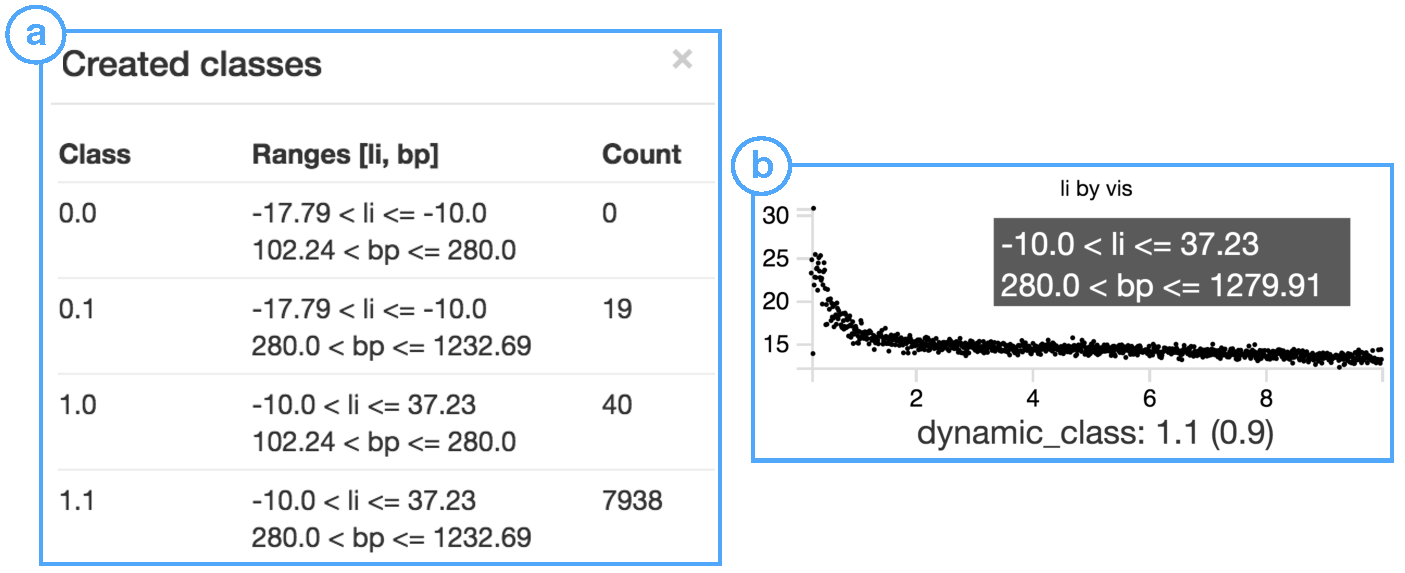
\includegraphics[width=\linewidth]{figures/dcc_example.pdf}
\vspace{-6pt}
\caption{Example of dynamic classes. (a) Four different classes with different Lithium solvation energies (li) and boiling point (bp) attributes based on user-defined data ranges. (b) Users can hover over the visualizations for each dynamic class to see the corresponding attribute ranges for each class. The visualizations of dynamic classes are aggregate across all the visualizations that lie in that class based on the user-selected aggregation method.}
\label{dcc}
\vspace{-10pt}
\end{figure}
%%%%%%%%%%%%%%%%%%%%%%%%%%%%%%%%%
\subsection{Finer System-level Control and  Understanding}
\par During the participatory design exercise, we found that many of the features suggested by the participants indicated they wanted finer control of the system. Prior work in direct manipulation visual interfaces has suggested that finer-grained control enabled users to discover patterns and rapidly generate hypothesis based on visual feedback \cite{Shneiderman1994,Shneiderman2007a}. 

\stitle{\tvcg{Controlling VQS internals:}}
In addition to query and dataset specifications, users also wanted the ability to modify the model parameters in \zv. Our findings echoed Chuang et al.~\cite{Chuang2012}, which showed that the ability to modify the model can facilitate interpretation and trust in model-driven visualizations, especially during early-stage exploration. These model parameter options include the ability to change the choice of similarity metrics (Figure \ref{zvOverview}j), the cluster size in the representative patterns (Figure \ref{zvOverview}k), setting a minimum similarity threshold for displaying the search results (Figure \ref{zvOverview}l), and the ability to tune the smoothing algorithm and parameter (Figure \ref{zvOverview}a).

\stitle{\tvcg{Displaying interpretable explanations for VQS recommendations:}} 
Explanatory system outputs include displaying similarity scores of the outputs, the number of datapoints in each cluster, and overlaying the original query sketch on the return visualization for comparison (Figure \ref{zvOverview}m). We further provided display-related options for plotting modifications, including displaying error bars, and toggling between a scatterplot and line chart view, to help analysts better understand the visualizations.